%%%%%%%%%%%%%%%%%%%%%%%%%%%%%%%%%%%%%%%%%%%%%%%%%%%%%%%%%%%%%%%%%%% 
%                                                                 %
%                            CHAPTER                              %
%                                                                 %
%%%%%%%%%%%%%%%%%%%%%%%%%%%%%%%%%%%%%%%%%%%%%%%%%%%%%%%%%%%%%%%%%%% 
 
\chapter{Implementation}
In this chapter, we will discuss the implementation. We introduce the shell dataset we created ourselves and establish a baseline with OWL-ViT. 

\section{Dataset}
In this section, we will go over the few-shot shell dataset we are introducing ourselves.

\subsection{Shells}

The shell dataset is a new dataset we are introducing ourselves. The images were taken with a cellphone camera on the Belgian coast. Each image has a size of 6144x8192px. Due to limited resources, the dataset is quite small, containing only 96 annotated images and 206 unannotated images. The images are annotated with bounding boxes of 8 types of shells, with 614 annotations in total. An overview of the annotations per class can be found in Table \ref{tab:shell_annotations}. The images are mostly sparse, with 1 to 3 shells per image. A limited amount of denser images is also present. A graph of the annotations per image in the dataset can be found in Figure \ref{fig:annotations_per_img}. Some examples of the images in the dataset can be found in table \ref{tab:shell_examples}.

%annotations: {
%     "Baltic tellin": 69,
%     "Cockle": 89,
%     "Thick trough shell": 91,
%     "Mussel": 268,
%     "Banded wedge shell": 32,
%     "Elliptical trough shell": 18,
%     "Cut trough shell": 36,
%     "Oyster": 9
% }

\begin{table}[H]
    \centering
    \captionsetup{justification=centering}
    \begin{tabular}{|l|l|}
    \hline
    \textbf{Shell type} & \textbf{Number of annotations} \\ \hline
    Baltic tellin       & 69                             \\ \hline
    Cockle              & 89                             \\ \hline
    Thick trough shell  & 91                             \\ \hline
    Mussel              & 268                            \\ \hline
    Banded wedge shell  & 32                             \\ \hline
    Elliptical trough shell & 18                         \\ \hline
    Cut trough shell    & 36                             \\ \hline
    Oyster              & 9                              \\ \hline
    \end{tabular}
    \caption{Overview of the annotations per class in the shell dataset.}
    \label{tab:shell_annotations}
\end{table}

\begin{figure}[H]
    \centering
    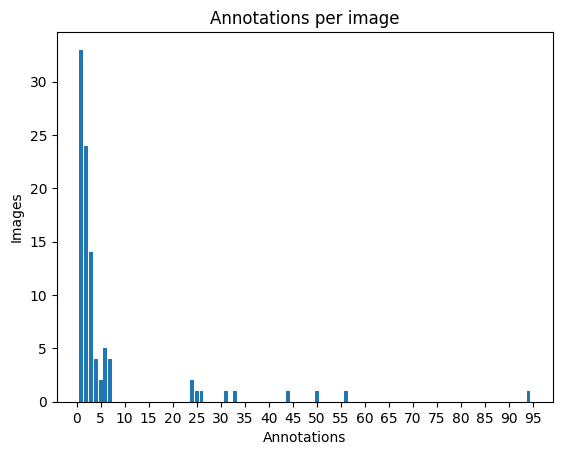
\includegraphics[width=0.8\textwidth]{chapter3/annotations_per_img.png}
    \caption{Overview of the annotations per image in the shell dataset.}
    \label{fig:annotations_per_img}
\end{figure}

\begin{figure}[H]
    \centering
    \captionsetup{justification=centering}
    \includegraphics[width=0.3\textwidth]{chapter3/shell_examples/1.jpg} 
    \includegraphics[width=0.3\textwidth]{chapter3/shell_examples/2.jpg} 
    \includegraphics[width=0.3\textwidth]{chapter3/shell_examples/3.jpg}
    \includegraphics[width=0.3\textwidth]{chapter3/shell_examples/4.jpg} 
    \includegraphics[width=0.3\textwidth]{chapter3/shell_examples/5.jpg} 
    \includegraphics[width=0.3\textwidth]{chapter3/shell_examples/6.jpg}
    \rotatebox{90}{\includegraphics[height=0.3\textwidth]{chapter3/shell_examples/7.jpg}} \rotatebox{90}{\includegraphics[height=0.3\textwidth]{chapter3/shell_examples/8.jpg}} \rotatebox{90}{\includegraphics[height=0.3\textwidth]{chapter3/shell_examples/9.jpg}} 
    \caption{Examples of images in the shell dataset.}
    \label{tab:shell_examples}
\end{figure}

\section{Baseline}
In this section, we establish a baseline for the shell dataset. For this, we will study the performance of OWL-ViT with image-based one-shot detection. 

\subsection{Model}
For the baseline, we will use the OWL-ViT model which is described in Section \ref*{sec:2_owlvit}. At inference time embeddings are extracted from the image using the ViT encoder. These object image embeddings are then compared to the query (text or image) embeddings as shown in figure \ref{fig:2_owl-vitr} to obtain a similarity score. The model exists in different flavors, with different backbones and different patch sizes. Hardware limitations limit us to the smallest ViT-B/32 model.

The model is implemented using the Scenic library \citep{scenic}. 
It is also included in the transformers library, which offers an abstraction layer for running the model. Running the model is done by loading the processor and model, using the processor on the query images and test image to obtain the inputs for the model and then running the model.

\subsection{Inference}
Setting up for inference follows the following steps:
\begin{enumerate}
    \item Load the model and processor.
        \begin{itemize}
            \item The model and processor are readily available from the transformers library.
        \end{itemize}
    \item Load the images and annotations.
        \begin{itemize}
            \item The images are Pascal VOC annotated, they are loaded into a class that offers the needed functionality.
        \end{itemize}
    \item Extract a query image for each class from the annotated images.
        \begin{itemize}
            \item The query images are extracted from the first image that contains an annotation of that class.
            \item Optionally the images can be shuffled to obtain a different query image for each class.
            \item The image from which the query image was taken is then removed from the test set. 
        \end{itemize}
    \item (Optional) Remove the background from the query images.
        \begin{itemize}
            \item The background is removed using the rembg library, which uses a neural network (u2net) to remove the background.
        \end{itemize}
\end{enumerate}
Inference is then done by doing image-guided detection with all the query images on each of the test images sequentially due to limited VRAM. 

\subsection{Processing}

Before interpreting the results, we can filter out unwanted detections. 

A common filter is to remove overlapping detections, with non-maximum suppression (NMS). This is done by removing all detections that have an IoU (intersection over union) with a higher scoring detection above a certain threshold. This threshold can be varied to see the impact on the results.

We also noticed that the model detects a large amount of excessively large boxes. As these detections are nearly guaranteed to be wrong and they can have a large impact on the results, we can filter them out by removing all detections that have a size larger than a certain threshold. This threshold is chosen relative to the size of the annotations, with the base value being set as the maximum size of the annotations after outlier rejection. This threshold can also be varied to see the impact on the results. 

We test the aforementioned filters with the following parameters:
\begin{itemize}
    \item NMS IoU threshold [0.1, 0.2, ..., 0.9, 1.0(no NMS)]
    \item Filtering excessively large boxes [relative to the size of the annotations * [0.75, 1, 2, 5]]
\end{itemize}
To find the optimal parameters, we calculate the mean average precision (mAP) and F1 score for each combination. The PR curves for each combination are plotted in figure \ref{fig:3_pr_curves_all_options}. The optimal parameters are the same for both mAP and F1 scores, with an NMS IoU threshold of 1 and a large box filter of 1. We get optimal results when we do no NMS and filter large boxes with the default threshold. To see the impact of NMS and large boxes filter threshold we set one value to their optimal value and plot the PR curves when varying the other. This results in Figure \ref{fig:3_pr_curves_nms} and Figure \ref{fig:3_pr_curves_large_boxes}.

% pr curves for all options
\begin{figure}[h]
    \centering
    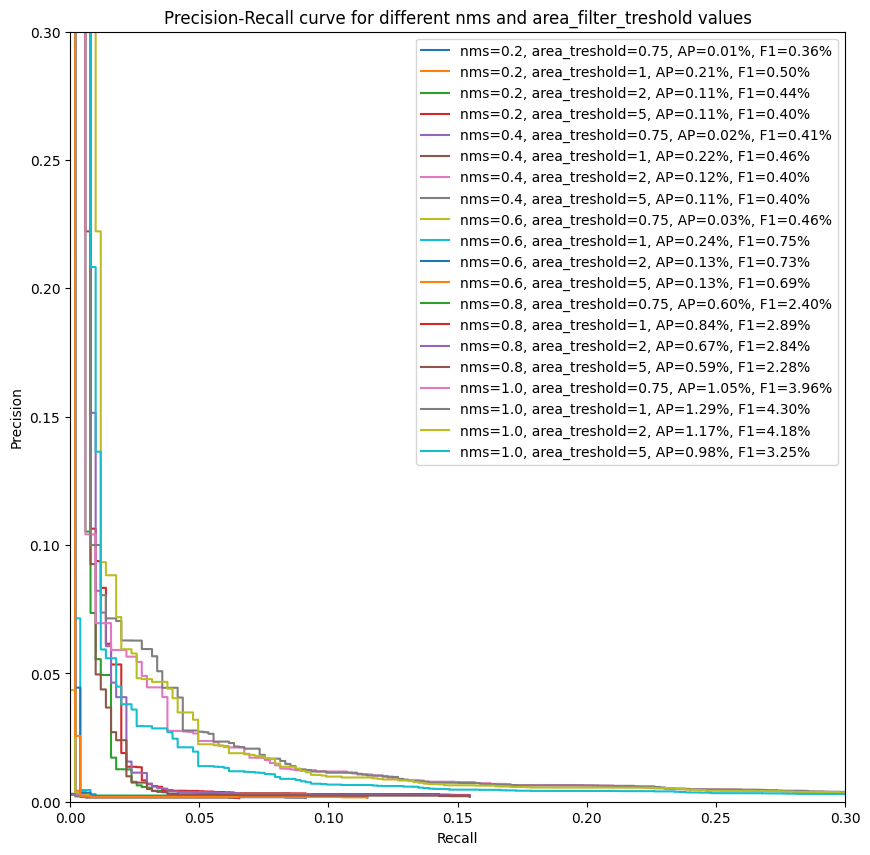
\includegraphics[width=1\textwidth]{chapter3/owl-vit/PR_all_options.png}
    \caption{PR curves for all options.}
    \label{fig:3_pr_curves_all_options}
\end{figure}

% pr curves for nms
\begin{figure}[h]
    \centering
    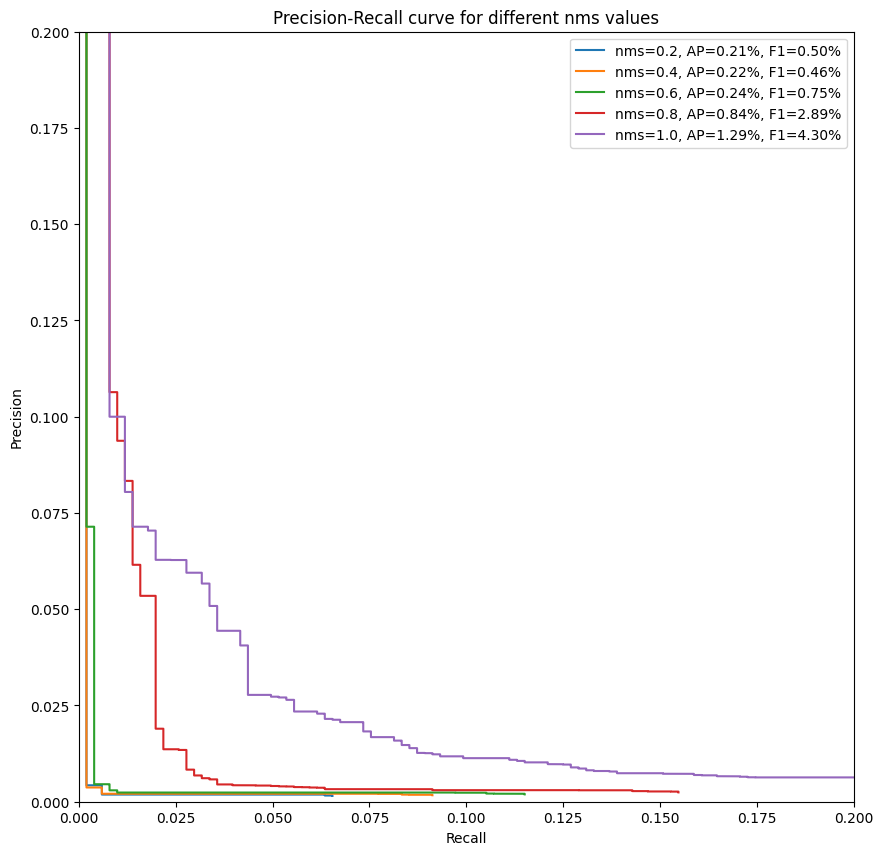
\includegraphics[width=0.7\textwidth]{chapter3/owl-vit/PR_all_nms.png}
    \caption{PR curves for different NMS IoU thresholds.}
    \label{fig:3_pr_curves_nms}
\end{figure}

% pr curves for large boxes
\begin{figure}[h]
    \centering
    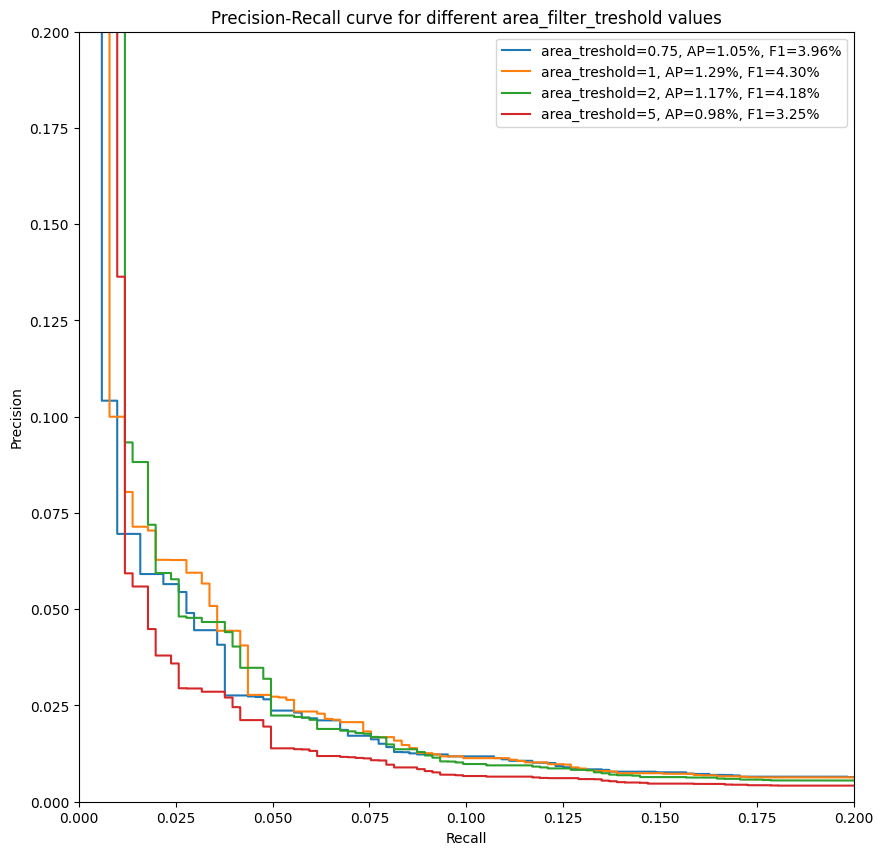
\includegraphics[width=0.7\textwidth]{chapter3/owl-vit/PR_all_areas.png}
    \caption{PR curves for different large boxes filter thresholds.}
    \label{fig:3_pr_curves_large_boxes}
\end{figure}

\subsection{Results}
Using the optimal values we found in the previous section, we can plot the PR curve and calculate the mAP and F1 score. Some visualizations of outputs are shown in Figure \ref{fig:3_outputs}. The PR curve is shown in Figure \ref{fig:3_optimal}. With a mAP of 1.29\% and a F1 score of 4.30\%, we can conclude that the baseline model is not able to reliably detect the objects in the shell dataset. We can do the above steps, but without comparing classes for the annotations and detections. This obtains the best score with an NMS threshold of 0.95, with differing values for the large boxes filter threshold depending on whether we optimize for the mAP or F1 score. The PR curves for these are shown in Figure \ref{fig:3_pr_curves_all_options_no_class_comparison}.

\begin{figure}[h]
    \begin{adjustwidth}{-1in}{-1in}
        \centering
        \includegraphics[width=0.3\pdfpagewidth]{chapter3/owl-vit/outputs/1.jpg}
        \includegraphics[width=0.3\pdfpagewidth]{chapter3/owl-vit/outputs/2.jpg}
        \includegraphics[width=0.3\pdfpagewidth]{chapter3/owl-vit/outputs/3.jpg}
        \includegraphics[width=0.3\pdfpagewidth]{chapter3/owl-vit/outputs/4.jpg}
        \includegraphics[width=0.3\pdfpagewidth]{chapter3/owl-vit/outputs/5.jpg}
        \includegraphics[width=0.3\pdfpagewidth]{chapter3/owl-vit/outputs/6.jpg}
        \rotatebox{90}{\includegraphics[height=0.3\pdfpagewidth]{chapter3/owl-vit/outputs/7.jpg}}
        \rotatebox{90}{\includegraphics[height=0.3\pdfpagewidth]{chapter3/owl-vit/outputs/8.jpg}}
        \rotatebox{90}{\includegraphics[height=0.3\pdfpagewidth]{chapter3/owl-vit/outputs/9.jpg}}
        \captionsetup{belowskip=-\baselineskip}
    \end{adjustwidth}
    \caption{Outputs of the baseline model with optimal parameters.}
    \setlength\belowcaptionskip{\baselineskip}
    \caption*{The filled boxes are annotations, and empty boxes are detections.}
    \label{fig:3_outputs}
\end{figure}

% pr curve for optimal
\begin{figure}[h]
    \centering
    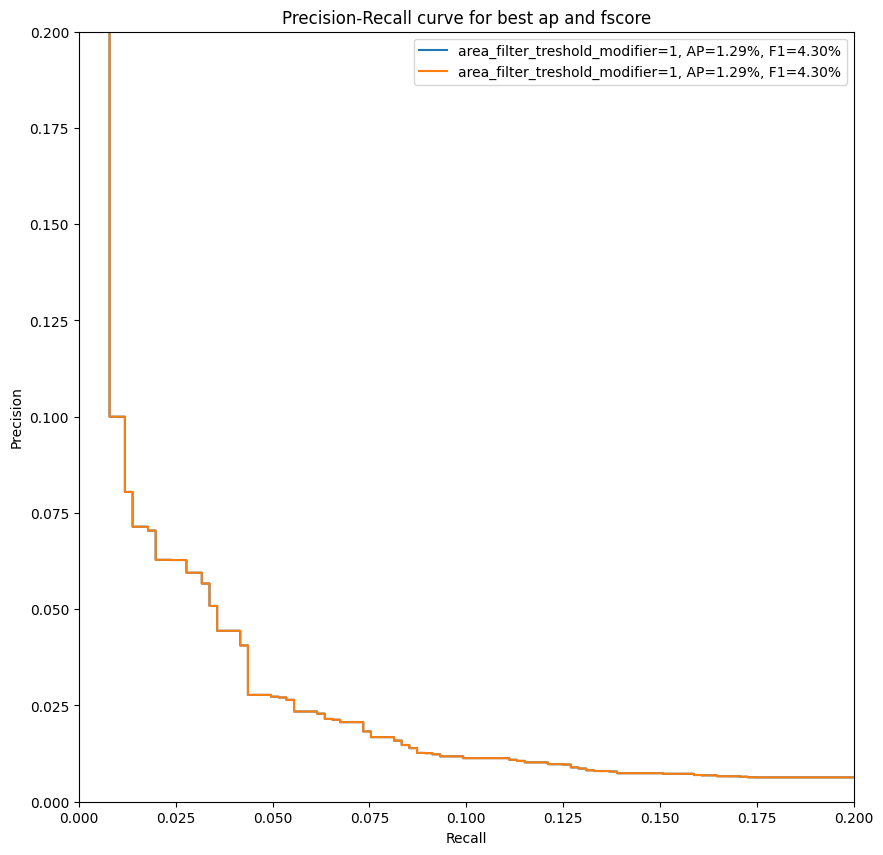
\includegraphics[width=0.7\textwidth]{chapter3/owl-vit/PR_optimal.png}
    \caption{PR curve for optimal parameters.}
    \label{fig:3_optimal}
\end{figure}

% pr curves for all options no class comparison
\begin{figure}[h]
    \centering
    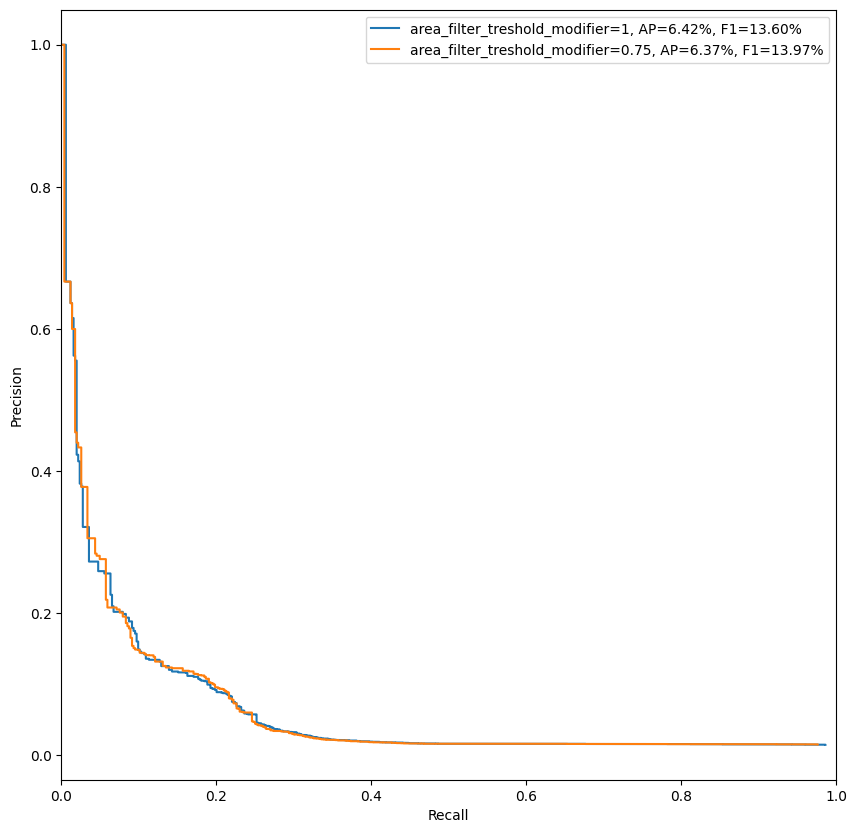
\includegraphics[width=1\textwidth]{chapter3/owl-vit/PR_no_class.png}
    \caption{PR curves for all options without comparing classes.}
    \label{fig:3_pr_curves_all_options_no_class_comparison}
\end{figure}

\subsection{Discussion}
The baseline model is not able to reliably detect the objects in the shell dataset. This is likely due to a combination of the following factors:
\begin{itemize}
    \item The model's training data likely has a limited representation of different types of shells. The training data is not publicly available, so we cannot verify this. The absence of specialised datasets for shells does however suggest this.
    \item The test data only has annotations for complete shells which are identifiable. The model detects many fragments or mostly buried shells, which are not annotated. This means that the model is penalized for detecting these shells, even though the detections might not be entirely wrong.
    \item We are using a basic version of the model, while larger versions are available. These larger versions perform better but require more performant hardware. This would make a difference, but we do not expect it to be large enough to make the model perform well.
\end{itemize}

\section{Conclusion}
In this thesis, we explored the SOTA in one-shot object detection to find if it is performant enough to count shells in an uncontrolled environment. We found that the current SOTA in one-shot object detection detects too many false positives and has a hard time differentiating between different types of shells. While some improvements can be made, we do not expect these to be large enough to make the model perform well. We conclude that the current SOTA in one-shot object detection is not able to reliably detect shells in an uncontrolled environment. 

\section{Future work}
We explored one-shot object detection for counting shells in an uncontrolled environment. We found that the current SOTA in one-shot object detection is not able to reliably detect shells in an uncontrolled environment. We propose the following future work to improve on this:
\begin{itemize}
    \item Use a K-shot, where the model has more than one image of each class available. This would allow the model to obtain a more complete representation of each type of shell.
    \item Use a trained model. The model we used did no finetuning, making it not optimized for our use case. In our case the classes we want to detect are very similar to each other, finetuning the model should allow it to differentiate better.
\end{itemize}